% !TeX document-id = {f19fb972-db1f-447e-9d78-531139c30778}
% !BIB program = biber

%\documentclass[handout]{beamer}
\documentclass[compress]{beamer}
\usepackage[T1]{fontenc}
\usetheme[block=fill,subsectionpage=progressbar,sectionpage=progressbar]{metropolis} 
\usepackage{graphicx}

\usepackage{wasysym}
\usepackage{etoolbox}
\usepackage[utf8]{inputenc}

\usepackage{pifont}

\usepackage{threeparttable}
\usepackage{subcaption}

\usepackage{tikz-qtree}
\usepackage{neuralnetwork}

\setbeamercovered{still covered={\opaqueness<1->{5}},again covered={\opaqueness<1->{100}}}


\usepackage{listings}

\lstset{
	basicstyle=\scriptsize\ttfamily,
	columns=flexible,
	breaklines=true,
	numbers=left,
	%stepsize=1,
	numberstyle=\tiny,
	backgroundcolor=\color[rgb]{0.85,0.90,1}
}



\lstnewenvironment{lstlistingoutput}{\lstset{basicstyle=\footnotesize\ttfamily,
		columns=flexible,
		breaklines=true,
		numbers=left,
		%stepsize=1,
		numberstyle=\tiny,
		backgroundcolor=\color[rgb]{.7,.7,.7}}}{}


\lstnewenvironment{lstlistingoutputtiny}{\lstset{basicstyle=\tiny\ttfamily,
		columns=flexible,
		breaklines=true,
		numbers=left,
		%stepsize=1,
		numberstyle=\tiny,
		backgroundcolor=\color[rgb]{.7,.7,.7}}}{}


% color-coded listings; replace those above 
\usepackage{xcolor}
\usepackage{minted}
\definecolor{listingbg}{rgb}{0.87,0.93,1}
\setminted[python]{
	frame=none,
	framesep=1mm,
	baselinestretch=1,
	bgcolor=listingbg,
	fontsize=\scriptsize,
	linenos,
	breaklines
	}


\usepackage[american]{babel}
\usepackage{csquotes}
\usepackage[style=apa, backend = biber]{biblatex}
\renewcommand*{\bibfont}{\tiny}


\usepackage{tikz}
\usetikzlibrary{shapes,arrows,matrix}
\usepackage{multicol}

\usepackage{subcaption}

\usepackage{booktabs}
\usepackage{graphicx}



\makeatletter
\setbeamertemplate{headline}{%
	\begin{beamercolorbox}[colsep=1.5pt]{upper separation line head}
	\end{beamercolorbox}
	\begin{beamercolorbox}{section in head/foot}
		\vskip2pt\insertnavigation{\paperwidth}\vskip2pt
	\end{beamercolorbox}%
	\begin{beamercolorbox}[colsep=1.5pt]{lower separation line head}
	\end{beamercolorbox}
}
\makeatother





\setbeamercolor{section in head/foot}{fg=normal text.bg, bg=structure.fg}


\newcommand{\instruction}[1]{\emph{\textcolor{gray}{[#1]}}}



\newcommand{\question}[1]{
	\begin{frame}[plain]
	\begin{columns}
		\column{.3\textwidth}
		\makebox[\columnwidth]{
			
\includegraphics[width=\columnwidth,height=\paperheight,keepaspectratio]{mannetje.png}}
		\column{.7\textwidth}
		\large
		\textcolor{orange}{\textbf{\emph{#1}}}
	\end{columns}
\end{frame}}


\tikzstyle{block} = [rectangle, draw, fill=blue!20, 
text width=5em, text centered, rounded corners, minimum height=4em]
\tikzstyle{line} = [draw]
\tikzstyle{pijltje} = [draw, -latex']
\tikzstyle{cloud} = [draw, ellipse,fill=red!20, node distance=3cm,
minimum height=2em, text width=4em, text centered,]


\setbeamercovered{transparent}

\addbibresource{../../resources/literature.bib}
\graphicspath{{../../resources/img/}}

\begin{document}

\title[Big Data and Automated Content Analysis]{\textbf{Big Data and Automated Content Analysis (6EC)} 
\\Week 1: »Programming for Computational (Communication\textbar Social) Scientists«
\\Monday }
\author[Anne Kroon]{Anne Kroon\\ \footnotesize{a.c.kroon@uva.nl}}
\date{April 3, 2023}
\institute[UvA CW]{UvA RM Communication Science}


\begin{frame}{}
	\titlepage
\end{frame}

\begin{frame}{Today}
	\tableofcontents
\end{frame}

\section{Getting to know each other}

\begin{frame}{Anne}

	\begin{columns}
		\column{.3\textwidth}
		\makebox[\columnwidth]{
			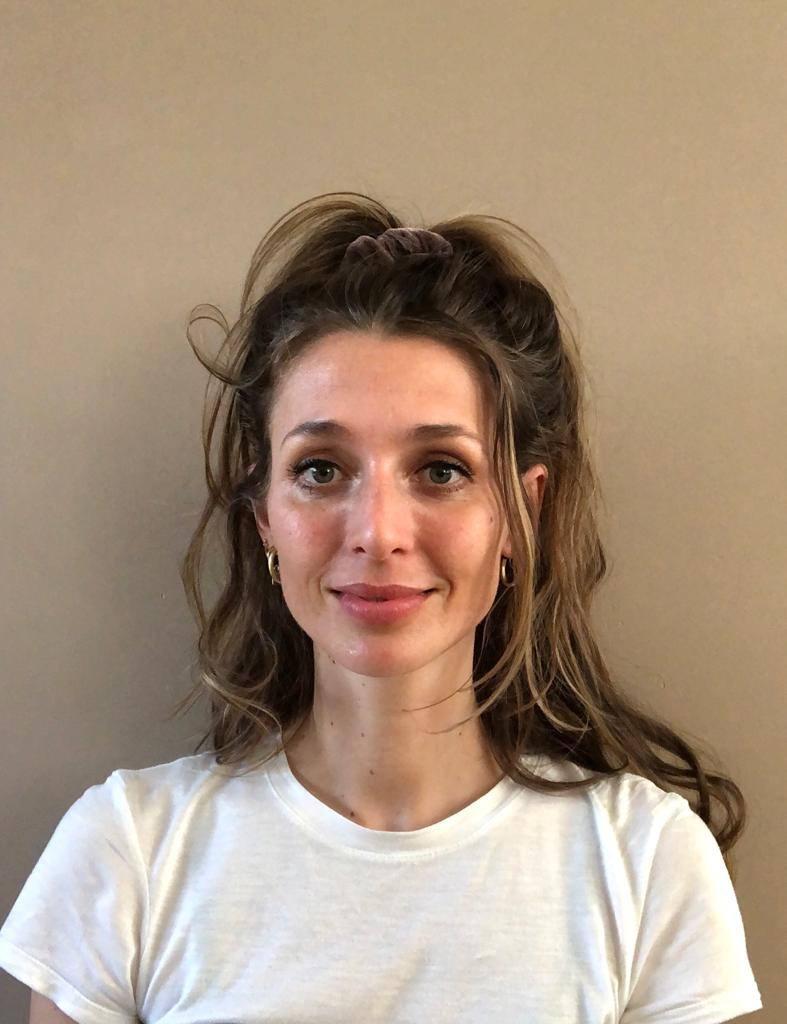
\includegraphics[width=\columnwidth,height=\paperheight,keepaspectratio]{anne.jpeg}}
		\column{.7\textwidth}
		dr. Anne Kroon \\
		Assistant Professor Corporate Communication \\
		\begin{itemize}
			\item studied Journalism (HU) and Communication Science at the UVA 
			\item PhD candidate @ ASCoR 2014--2017
			\item bias in media representations of minorities, algorithmic bias in hiring and selection 
			\item computational research methods
		\end{itemize}
		@annekroon ~~ a.c.kroon@uva.nl ~~ REC-C~7\textsuperscript{th}~floor 
	\end{columns}
\end{frame}


\begin{frame}{You}
	\begin{columns}
		\column{.3\textwidth}
		\makebox[\columnwidth]{
			
\includegraphics[width=\columnwidth,height=\paperheight,keepaspectratio]{mannetje.png}}
		\column{.7\textwidth}
		Your name?\\
		Your background?\\
		Your reason to follow this course?
	\end{columns}
\end{frame}


\section[What is CSS\textbar CCS?]{What is computational \lbrack social\textbar communication\rbrack  ~science?}

%What is computational \lbrack social\textbar communication\rbrack  ~science?



\subsection{Defining CCS}



\begin{frame}{A very young field}
	\begin{block}{\textcite{Lazer2009}}
		``The capacity to collect and analyze massive amounts of data has transformed such fields as biology and physics. But the emergence of a data-driven `computational social science' has been much slower.''
	\end{block}
\end{frame}




\begin{frame}{Epistemologies and paradigm shifts}
	\begin{block}{\textcite{Kitchin2014}}<1->
		\begin{itemize}
			\item<2-> (Reborn) empiricism: purely inductive, correlation is enough
			\item<3-> Data-driven science: knowledge discovery guided by theory
			\item<4-> Computational social science and digital humanities: employ Big Data research within existing epistemologies
			\begin{itemize}
				\item DH: descriptive statistics, visualizations
				\item CSS: prediction and simulation
			\end{itemize}
		\end{itemize}
	\end{block}
\end{frame}




\begin{frame}{CCS as a subset of CSS}
	\begin{block}{\textcite{Hilbert2019}}
		``\ldots our definition of computational communication science as an application of computational science to questions of human and social communication. As such, it is a natural subfield of computational social science'' (followed by references to CSS definitions)
	\end{block}
\end{frame}



\begin{frame}{Data, analysis, theory}
	\begin{block}{\textcite{VanAtteveldt2018a}}
		``\ldots computational communication science studies generally involve: (1) large and complex data sets; (2) consisting of digital traces and other ``naturally occurring'' data; (3) requiring algorithmic solutions to analyze; and (4) allowing the study of human communication by applying and testing communication theory.''
	\end{block}	
	
\end{frame}





\subsection{And Big Data?}

\begin{frame}[standout]
It was a buzzword when we first designed this course in 2013 (very much like ``AI'' and ``algorithm'' are today).

It's hard to define, but it can help us thinking about the characteristics of the data we deal with.
\end{frame}


\begin{frame}{The ``pragmatic'' definition }
	\begin{block}{}
		Everything that needs so much computational power and/or storage that you cannot do it on a regular computer.
	\end{block}
\end{frame}



\begin{frame}{The ``commercial'' definition }
	\begin{block}{\textcite{gartner}}
		``Big data is high-volume, high-velocity and/or high-variety information assets that demand cost-effective, innovative forms of information processing that enable enhanced insight, decision making, and process automation.''
	\end{block}
\end{frame}



\begin{frame}{The ``critical'' definition }
	\begin{block}{\textcite{boyd2012}}
		``
		\begin{enumerate}
			\item Technology: maximizing computation power and algorithmic accuracy to gather, analyze, link, and compare large data sets.
			\item Analysis: drawing on large data sets to identify patterns in order to make economic, social, technical, and legal claims.
			\item Mythology: the widespread belief that large data sets offer a higher form of intelligence and knowledge that can generate insights that were previously impossible, with the aura of truth, objectivity, and accuracy.
		\end{enumerate}
		''
	\end{block}
\end{frame}




\question{Do you think that now, a decade later, \citeauthor{boyd2012}'s argument is still valid? Or does it need to be adapted?}


\begin{frame}{We have become more critical about it!}
	Reading tips: \textcite{Bender2021, Bolukbasi2016}.
	
	These articles are about techniques using big datasets that we will talk about towards the end of this course, so it's OK if you don't understand them fully (yet).
\end{frame}


\question{
	\begin{enumerate}
		\item 	What do you think? What is the essence of Big Data/CSS/CCS?
		\item How will what we do here relate to theories and methods from other courses?
	\end{enumerate}
}





\subsection{The role of software in CSS}

\begin{frame}{CSS means also a shift in our relationship to software}
	In the (traditional) social sciences, we tend to think of software as\ldots
\begin{itemize}
	\item a monolithic block: a large standalone programme like Word or SPSS;
	\item something that either fulfills your needs or doesn't: it's often impossible, but at least uncommon and difficult, to adapt or change it;
	\item something with a graphical user interface;
	\item (often) something you pay for.
\end{itemize}
\end{frame}



\begin{frame}{CSS means also a shift in our relationship to software}
	In CSS, that's (typically) different:
	\begin{itemize}
		\item We mix and combine different ``modules'' or ``libraries'' ($\approx$ building blocks for programs)
		\item We build on modules made by others so that we don't reinvent the wheel, but ultimately build our own programs.
		\item We use a programming language to do all of this.
	\end{itemize}
\end{frame}






\begin{frame}{Why program your own tool?}
	\begin{block}{\textcite{Vis2013}}
		``Moreover, the tools we use can limit the range of questions that might be imagined, simply because they do not fit the affordances of the tool. Not many researchers themselves have the ability or access to other researchers who can build the required tools in line with any preferred enquiry. This then introduces serious limitations in terms of the scope of research that can be done.''	
	\end{block}
	
\end{frame}


\begin{frame}{Some considerations regarding the use of software in science}
	Assuming that science should be \emph{transparent} and \emph{reproducible by anyone}\onslide<2->{, we should}
	\begin{block}{use tools that are}<2->
		\begin{itemize}
			\item platform-independent 
			\item free (as in beer and as in speech, gratis and libre)
			\item which implies: open source
		\end{itemize}
	\end{block}
	\onslide<3>{This ensures it can our research (a) can be reproduced by anyone, and that there is (b) no black box that no one can look inside. $\Rightarrow$ ongoing open-science debate! \parencite{VanAtteveldt2019}}
\end{frame}

\begin{frame}{Why program your own tool?}
	\begin{block}{\textcite{Vis2013}}
		``{[}\ldots{]} these {[}commercial{]} tools are often unsuitable for academic purposes because of their cost, along with the problematic `black box' nature of many of these tools.''
	\end{block}
	
	\begin{block}{\textcite{Mahrt2013}}
		``{[}\ldots{]} we should resist the temptation to let the opportunities and constraints of an application or platform determine the research question {[}\ldots{]}''
	\end{block}
\end{frame}


\question{Do you think one \textit{needs} a programming language to do CSS? Why?}

\begin{frame}{So I need a programming language to do CSS?}

\begin{itemize}
	\item In principle, it does not matter \emph{which} programming language you use.
	\item \textbf{Python} and \textbf{R} are by far the most popular languages \emph{for CSS}
	\item But that may change: Nowadays, most scientific articles are written in English -- in some fields, that used to be Latin, German, Russian
\end{itemize}

\textbf{If you learn one programming language, it is relatively easy to learn another one.}
(Think of learning Spanish after you learned French)

\end{frame}


\section{What is Python?}

\subsection{Python: A language, not a program}


\begin{frame}[plain]
	\makebox[\columnwidth]{
		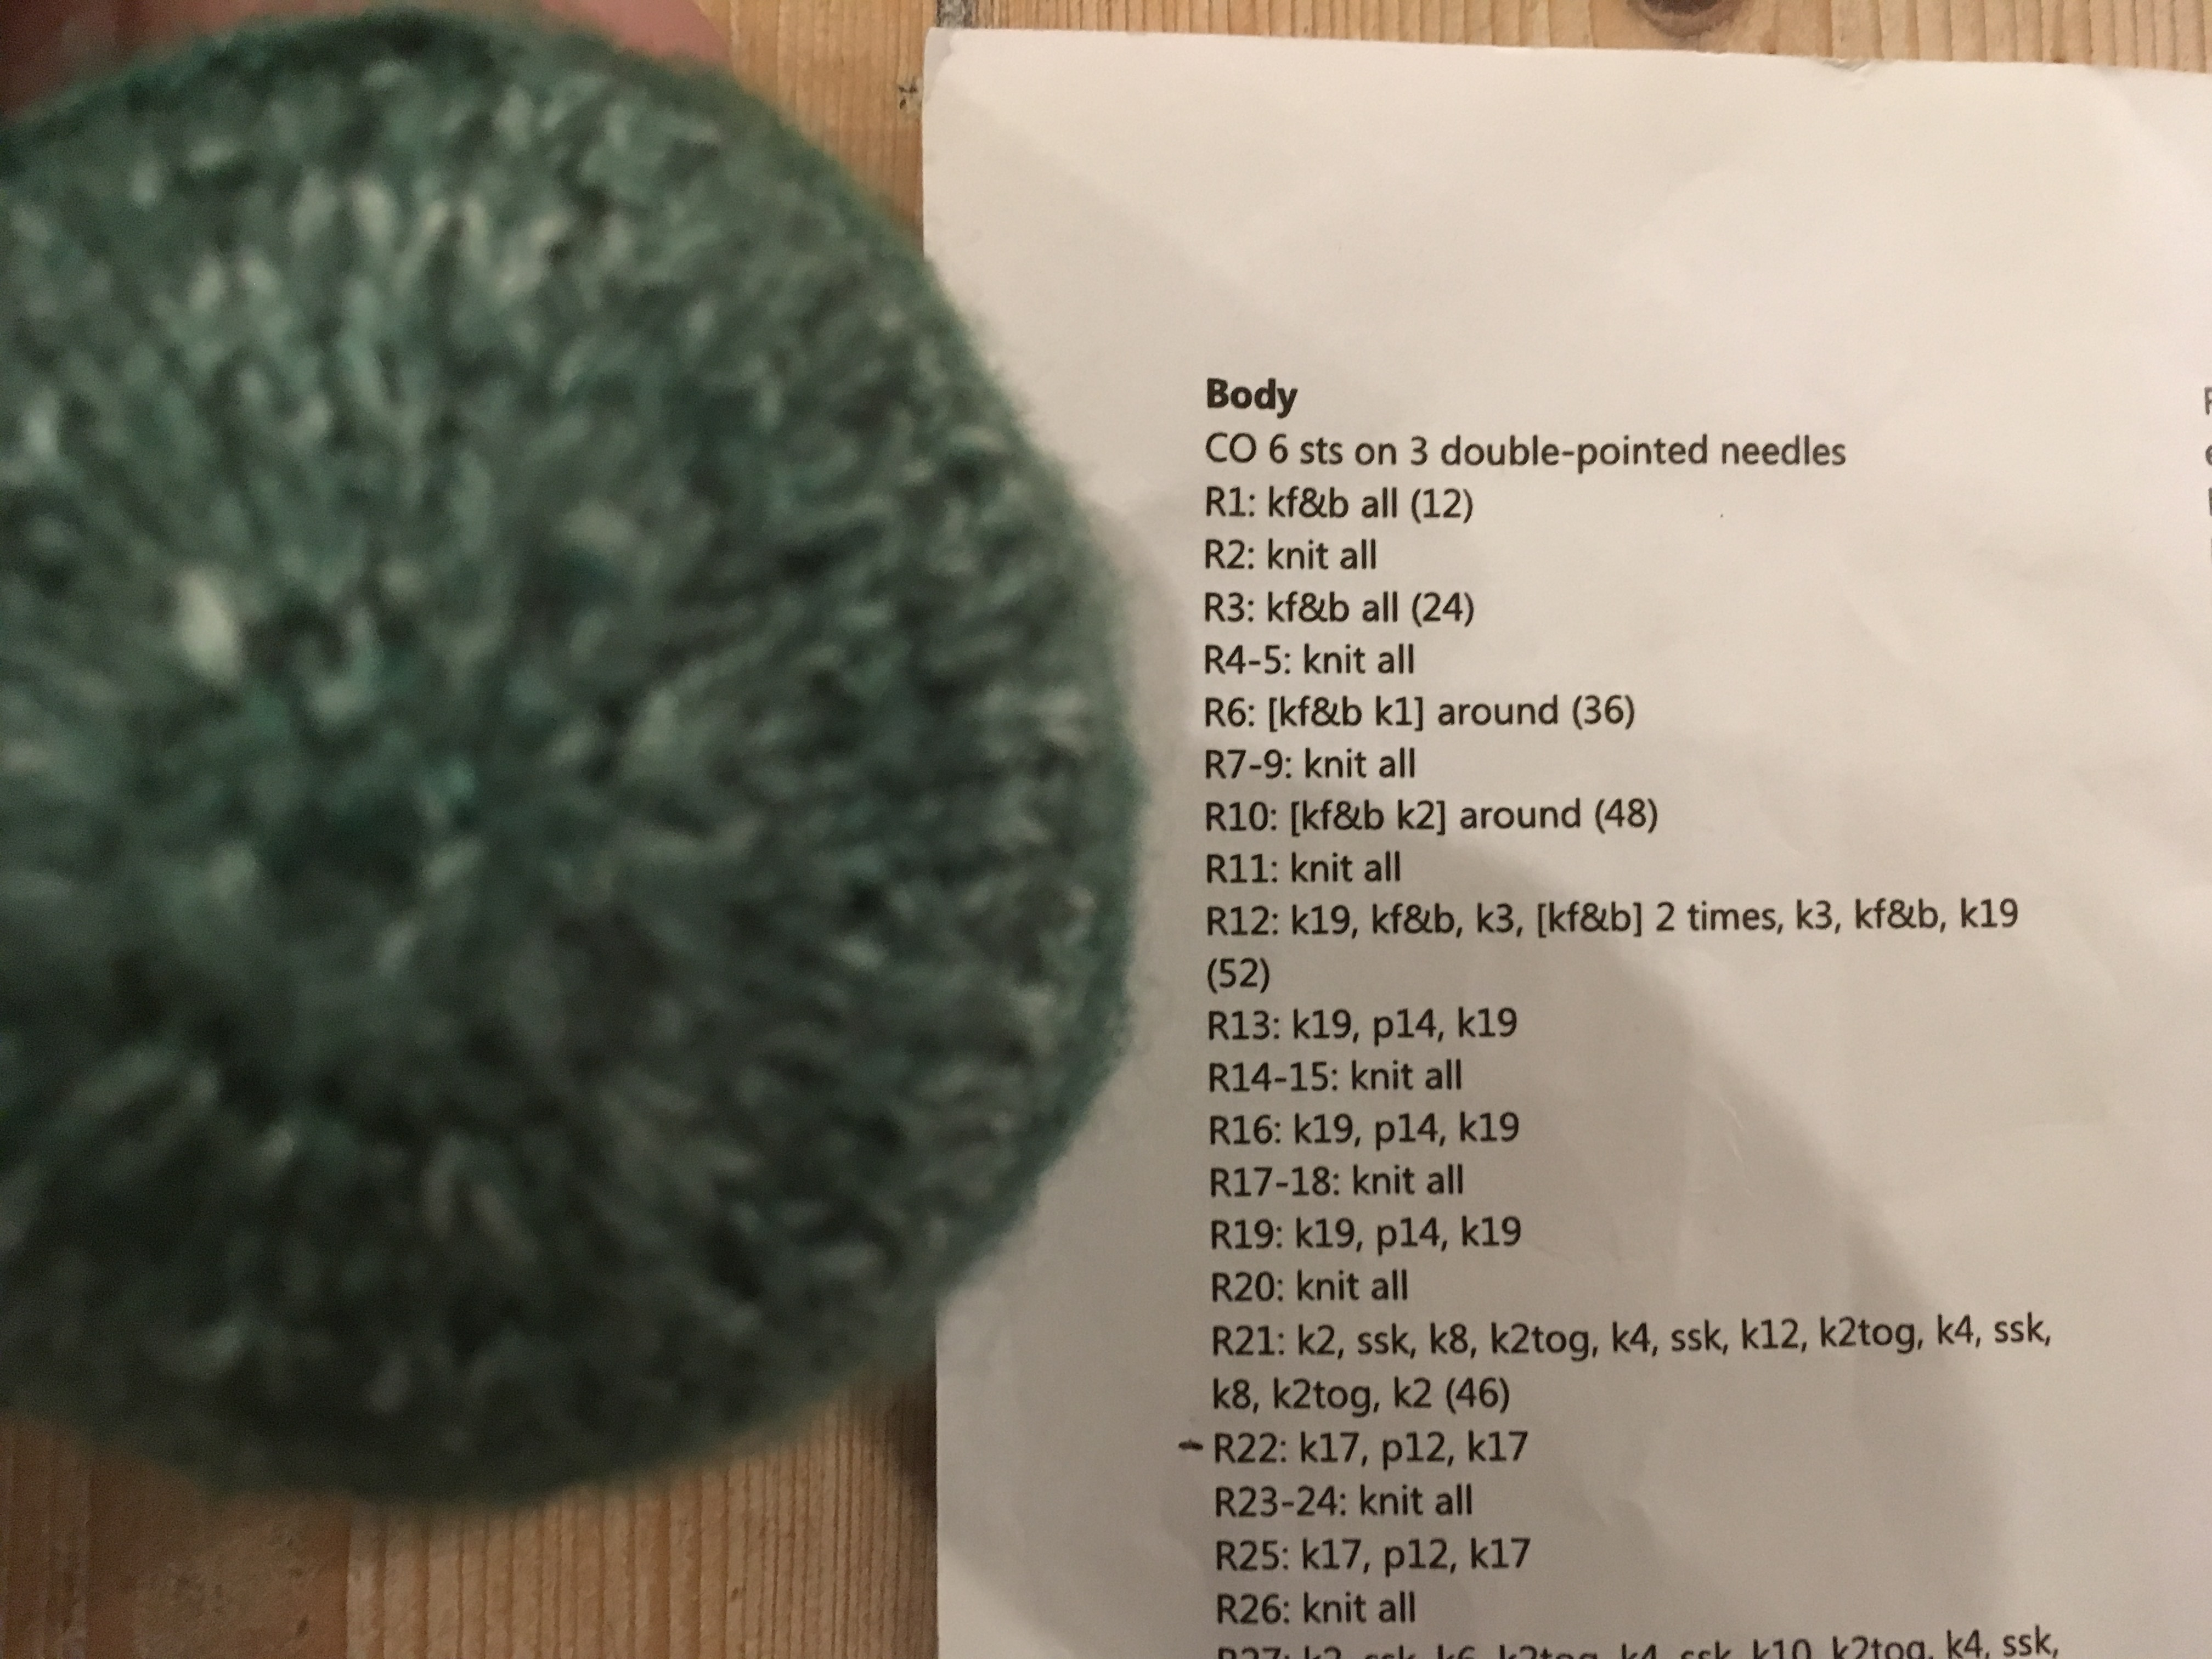
\includegraphics[width=\columnwidth,height=\paperheight,keepaspectratio]{knitting.jpg}}
	\footnotesize{An algorithm in a language that's a bit harder (I think) than Python}
\end{frame}



\begin{frame}{Python}
	\begin{block}{What?}<1->
		\begin{itemize}
			\item A language, not a specific program
			\item Huge advantage: flexibility, portability
			\item One of \emph{the} languages for CCS. \tiny{(The other one is R.)}
		\end{itemize}
	\end{block}
	
	\begin{block}{Which version?}<2->
		We use Python 3. (I use 3.8.10 right now, but with anything above 3.6 you're probably fine)\\ 
		You may occasionally still encounter Python2-code. One difference: In Python 2, you write {\tt print "Hi"} instead of {\tt print ("Hi")}.\\
	\end{block}
\end{frame}


\subsection{Python versus R}
\begin{frame}{Should I use Python or R?}
	\begin{itemize}
		\item For some people, an almost religious debate (but that's stupid!)
		\item Different history: R comes from math and statistics, Python from computer science
		\item Different user communities: statisticians: R, linguists: Python; most of industry: Python
		\item Nowadays (unlike some years ago), most things that are relevant to us can be done in \emph{both} languages.
	\end{itemize}
\pause
\textcolor{orange}{\textbf{Specialize in one language, but have a basic understanding of both!}}
\end{frame}


\begin{frame}{Should I use Python or R?}
	\begin{block}{For those of you who know R}
		You will notice a few things:
		\begin{itemize}[<+>]
			\item R ``abstracts away'' more stuff; in Python, you need to be a bit more explicit
			\item In R, (almost) everything is a dataframe or a vector, in Python not
			\item There is a big difference between applying a function to a single value or a whole ``column'' in Python
			\item In Python, we start counting with 0 (not 1)
		\end{itemize}

	\end{block}
\end{frame}


\begin{frame}{Should I use Python or R?}
	\begin{block}{For those of you who know R}
		You will notice a few things:
		\begin{itemize}[<+>]
			\item Typical ``user level'' R-code often is essentially written as consecutive commands: line for line. Structuring the code using typical programming constructs (writing own functions, using control strucutures) is not considered ``pro'' use (like in R), but \emph{the} way to work in Python.
			\item Python likes object orientation, R likes functions and pipelines
		\end{itemize}
		
	\end{block}
\end{frame}



\begin{frame}{Why do we use Python in this course?}
\begin{itemize}
	\item Python is a general programming language, R is a domain-specific one (it's meant for stats).
	\item The course is on ACA, and the closely related computational linguistics community uses Python.
	\item Python is \emph{much} better equipped for machine learning (and R for traditional stats, but that's not our focus).
	\item Web scraping is possible in R, but typically done in Python.
	\item If you know Python, you can probably learn many other languages quite quickly (including R). That's a bit more difficult coming from R.
\end{itemize}
	
\end{frame}



\begin{frame}{You can build \emph{anything}, including a live news aggregator!} 
	Beyond the scope of this course, but this was a Master thesis \parencite{3bij3}:
	\makebox[\columnwidth]{
		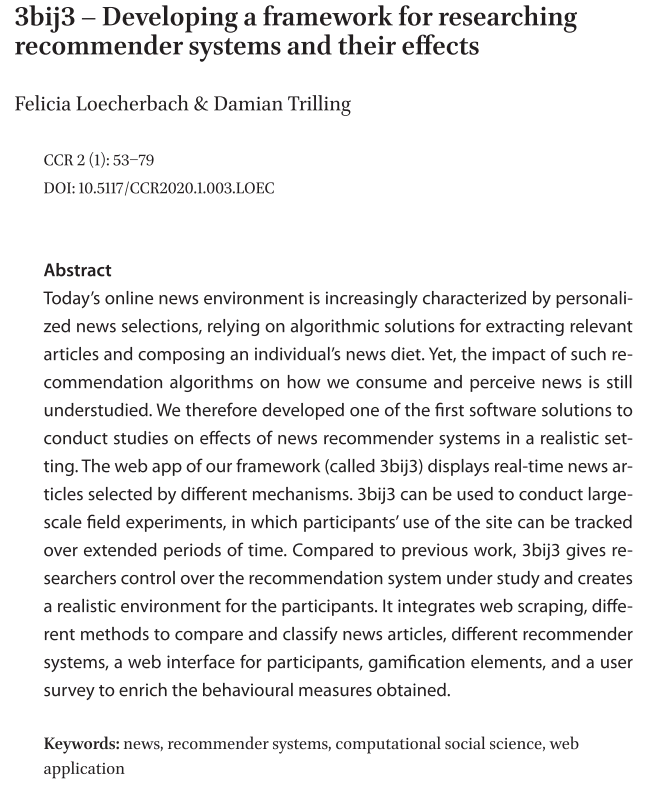
\includegraphics[width=\columnwidth,height=\paperheight,keepaspectratio]{3bij3article.png}}
\end{frame}


\begin{frame}[plain]
	\makebox[\columnwidth]{
		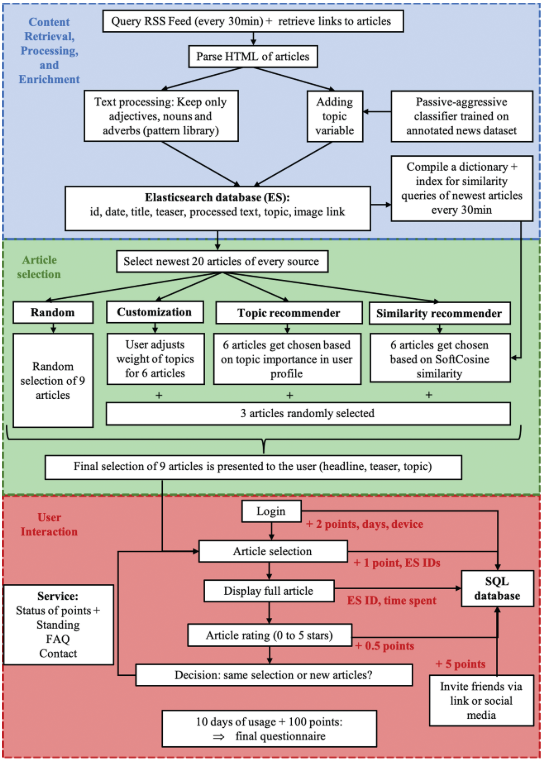
\includegraphics[width=\columnwidth,height=\paperheight,keepaspectratio]{3bij3article2.png}}
\end{frame}

\subsection{What do we need to write Python programs?}

\begin{frame}{1. A Python interpreter}
A Python interpreter -- a program that ``understands'' Python and translates it into low-level commands that your computer executes.

Type \texttt{python3} in your operating system's command line:

	\makebox[\columnwidth]{
	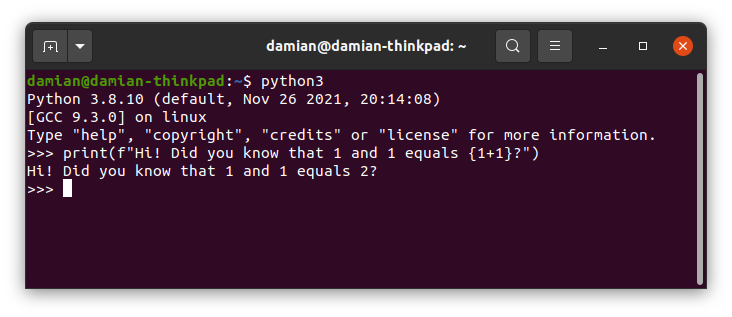
\includegraphics[width=.8\columnwidth,keepaspectratio]{repl.png}}
That's also called a Read-Evaluate-Print-Loop (REPL)
\end{frame}

\begin{frame}{2. Some more comfort}
\begin{itemize}[<+->]
	\item Starting an interpreter like this useful for quick try-outs, but not really a way to write full programs
	\item You can write them in a (good) text editor (Atom, Sublime, Notepad++, geany, emacs, vi) -- that's how it has historically been done and still a good skill to have
	\item But there are also \emph{Integrated Development Environments} (IDEs) that integrate an editor and an interpreter and offer a lot of extra funcitonality
	\item We will mainly work with Jupyter (which is tailored to data analyst's needs), but you you can consider checking out PyCharm or Visual Studio Code (both used by professional programmers) or Spyder (for those who like RStudio)
\end{itemize}
\end{frame}

\begin{frame}{3. Additional modules}
	\begin{itemize}
		\item A great advantage of Python are the many packages to extend it. 
		\item You can install them using a command called \texttt{pip}
		\item Alternatively, the Anaconda distribution already comes with most (but probably not all) you'll need pre-installed.
	\end{itemize}
\end{frame}

\question{You see why I talked about the difference between monolitic software like SPSS and the ``a language, not a program''-notion here?}


\section{Expectation Management}


\begin{frame}[standout]
	Let's talk a bit about what this course can and cannot offer, and what my and your expectations are.
\end{frame}


\begin{frame}{Expectation 1: The course materials can't offer everything.}
There is a lot of great stuff out there: YouTube tutorials, blogs, \ldots And I don't believe that the way I explain, say, Web Scraping is the one and only way to do it, for each and everyone.

In the end, it is about you learning something -- not about following exactly what I say. If you find a source that you think explains something better than I do: Use it! Share it!
\end{frame}


\begin{frame}{Expectation 2: Use Stackoverflow. But acknowledge your sources.}
%You'll quickly discover that googling a Python-related question usually takes you to StackOverflow.
Learn from other people's code and don't reinvent the wheel. But indicate in your assignments clearly where you got some code from! 

(Otherwise, I'll report you for plagiarism. And I don't want to do that.)
\end{frame}


\begin{frame}[standout]
I don't have to tell you that you can prompt ChatGPT to ``write a for loop in Python''. But next to this being fraud if you hand it in, it -- even more importantly -- won't teach you anything. Also, in case of suspicious code (e.g., code using very different idioms and approaches than we discussed), I'll reserve the right to question you to explain what's happening.
\end{frame}



\begin{frame}{Expectation 3: You have to practice.}
	You have to practice, preferably with a classmate. Try to modify the code we used, or write something (anything) on your own. Use the Thursday sessions to ask for feedback on that.
\end{frame}



\begin{frame}{Expectation 4: The first weeks are crucial.}
The first weeks are crucial, really. REALLY. REALLY!!!

Maybe quite counterintuitively, the fancy stuff we are doing later (Machine Learning\ldots) is relatively easy to do. But only if you know your basics %(as in: be able to explain Chapter 3 of the book in the middle of the night to your grandparents)

Want to take it easy some weeks? Better do so later in the course ;-)
\end{frame}


\begin{frame}{Expectation 5: You are an individual.}
\begin{itemize}
	\item There is wide variation of how quickly people ``get it'' in the first weeks. You are not stupid if it takes a bit longer!
	\item In the end, you will need to deliver an individual research project on a topic of your own choice.
	\item You should consult me on the exact scope, but it needs to include multiple techniques from both parts of the course.
	\item Some students say they prefer more standardized testing, but that would be \emph{in conflict with the main learning goal of this course}: Being able to conduct a CSS reseach project, from beginning to end.
	\item But most students actually find this one of the best things of this course, and so do I: It's great to read all your creative work!
\end{itemize}

\end{frame}


\begin{frame}{Structure of the meetings (usually)}
	\begin{description}
		\item[Monday] Lecture
		\item[Thursday]Lab session.
	\end{description}
See Course Manual for specific preparation and readings.

In general, we will work on some programming exercise \emph{during} the lab sessions, so that you can immediately ask questions when you get stuck.

No weekly assignments to hand in, but implicit continous assignment: Finish the exercises we do in class, and play with them/extend them/write your own code!
\end{frame}

\begin{frame}{Testing}
\begin{itemize}
	\item Two take-home exams and one individual project
	\item Reserve some time for the take-home exams (sometimes, it helps to sleep a night)
	\item In the exams, you need to program, but also have read the literature
	\item For details, see Course Manual
\end{itemize}
\end{frame}

\question{Any questions?}

\subsection{Next steps}


\begin{frame}[standout]
	Make sure you can run Python code and install packages. Otherwise, you won't be able to follow along on Thursday. (See instructions you got.)
\end{frame}


\begin{frame}[allowframebreaks,plain]
	\printbibliography
\end{frame}


\end{document}
